% Cronograma y presupuesto (cronograma.tex). El cronograma retoma las fechas
% del calendario de recolección del bosquejo del método
% (secciones/16-bosquejo-metodo.tex, Tabla tab:calendario-metodo) y del
% Apéndice D; si cambia una fecha, actualizar los tres archivos. Las fechas de
% entrega del protocolo son las \duedate de trabajo.tex. El desarrollo del
% prototipo (26 de octubre al 27 de noviembre) y los responsables vienen del
% plan de gestión (Niza/gestion/06-planificacion.tex y 07-equipo.tex).
% El presupuesto es el mismo del plan de gestión (Tabla tab:costos), con el
% desglose de lo que incluye cada partida; no se agregaron precios nuevos.
\section{Cronograma}
El cronograma ordena en el tiempo las actividades necesarias para responder
la pregunta de investigación. Abarca del 28 de septiembre de 2026 al 29 de
enero de 2027 y se divide en tres etapas. La primera es la elaboración del
protocolo, que ya concluyó con la entrega del bosquejo del método. La segunda
es el trabajo de campo: autorizaciones, aplicación de los instrumentos,
pruebas de banco y piloto en el acceso peatonal del \tescha{}. La tercera es
el análisis de los datos y la presentación de los resultados. Las fechas del
trabajo de campo son las del calendario de recolección del bosquejo del
método y del plan de acción del Apéndice~D.

La Tabla~\ref{tab:cronograma} presenta cada actividad con su periodo, su
responsable y el producto que deja, y la Figura~\ref{fig:gantt} muestra las
mismas actividades en un diagrama de Gantt.

\begin{table}[htbp]
	\caption{Cronograma de Actividades}
	\label{tab:cronograma}
	\small\linespread{1}\selectfont\setlength{\tabcolsep}{3pt}
	\begin{tabular}{@{}P{5.3cm}P{3.7cm}P{3cm}P{3.8cm}@{}}
		\toprule
		Actividad & Periodo & Responsable & Producto \\
		\midrule
		\multicolumn{4}{@{}l}{\textit{Etapa 1. Elaboración del protocolo}} \\[0.2em]
		Planteamiento del problema y objetivos & Entrega: 30 de septiembre de 2026 & Todo el equipo & Planteamiento y objetivos \\[0.4em]
		Justificación & Entrega: 15 de octubre de 2026 & Todo el equipo & Justificación \\[0.4em]
		Marco teórico & Entrega: 27 de octubre de 2026 & Todo el equipo & Marco teórico \\[0.4em]
		Hipótesis & Entrega: 12 de noviembre de 2026 & Todo el equipo & Hipótesis de investigación \\[0.4em]
		Bosquejo del método & Entrega: 17 de noviembre de 2026 & Todo el equipo & Bosquejo del método y Apéndices A a G \\[0.4em]
		\multicolumn{4}{@{}l}{\textit{Etapa 2. Trabajo de campo}} \\[0.2em]
		Desarrollo y ajuste del prototipo (hardware, lector y servidor) & 26 de octubre al 27 de noviembre de 2026 & Daniel Arellano, Ian Flores, Miguel Jurado y Juan Fernando Reyes & Prototipo integrado \\[0.4em]
		Solicitud de autorización a la Dirección y a Control Escolar & 18 al 20 de noviembre de 2026 & Juan Esteban Anzures & Oficio de solicitud \\[0.4em]
		Revisión de la legislación de protección de datos & 18 al 27 de noviembre de 2026 & Miguel Jurado & Ficha de requisitos (Apéndice~F) \\[0.4em]
		Prueba del cuestionario y de la hoja de observación & 23 y 24 de noviembre de 2026 & Bryan Villegas & Apéndices A y C corregidos \\[0.4em]
		Entrevistas a vigilancia y a Control Escolar & 23 al 27 de noviembre de 2026 & Bryan Villegas & Guía de entrevista (Apéndice~B) \\[0.4em]
		Aplicación de la encuesta & 25 de noviembre al 4 de diciembre de 2026 & Bryan Villegas & Cuestionario (Apéndice~A) \\[0.4em]
		Pruebas de banco del prototipo & 30 de noviembre al 4 de diciembre de 2026 & Ian Flores y Juan Fernando Reyes & Hoja de pruebas de banco (Apéndice~E) \\[0.4em]
		Primera serie de observación (línea base) & 30 de noviembre al 4 de diciembre de 2026 & Bryan Villegas & Hoja de observación (Apéndice~C) \\[0.4em]
		Instalación, alta de estudiantes y adaptación & 7 y 8 de diciembre de 2026 & Daniel Arellano y Juan Fernando Reyes & Consentimientos (Apéndice~G) \\[0.4em]
		Segunda serie de observación (piloto) & 9 al 15 de diciembre de 2026 & Bryan Villegas & Hoja de observación (Apéndice~C) \\[0.4em]
		\multicolumn{4}{@{}l}{\textit{Etapa 3. Análisis y resultados}} \\[0.2em]
		Procesamiento y análisis de los datos & 16 de diciembre de 2026 al 15 de enero de 2027 & Todo el equipo & Base de datos y resultados \\[0.4em]
		Presentación de resultados & 18 al 29 de enero de 2027 & Juan Esteban Anzures & Informe final \\
		\bottomrule
	\end{tabular}
	\tablenote{Elaboración propia a partir del calendario de recolección del
		bosquejo del método, del Apéndice~D y del plan de gestión del proyecto.
		Las fechas de la etapa 2 en adelante son una propuesta sujeta al
		calendario escolar, a la autorización del plantel y a que el prototipo
		pase las pruebas de banco. El receso del 21 de diciembre al 1 de enero
		no se cuenta.}
\end{table}

\begin{figure}[htbp]
	\caption{Diagrama de Gantt del Proyecto}
	\label{fig:gantt}
	\centering
	% x: días desde el lunes 28 de septiembre de 2026; y: una fila por actividad.
	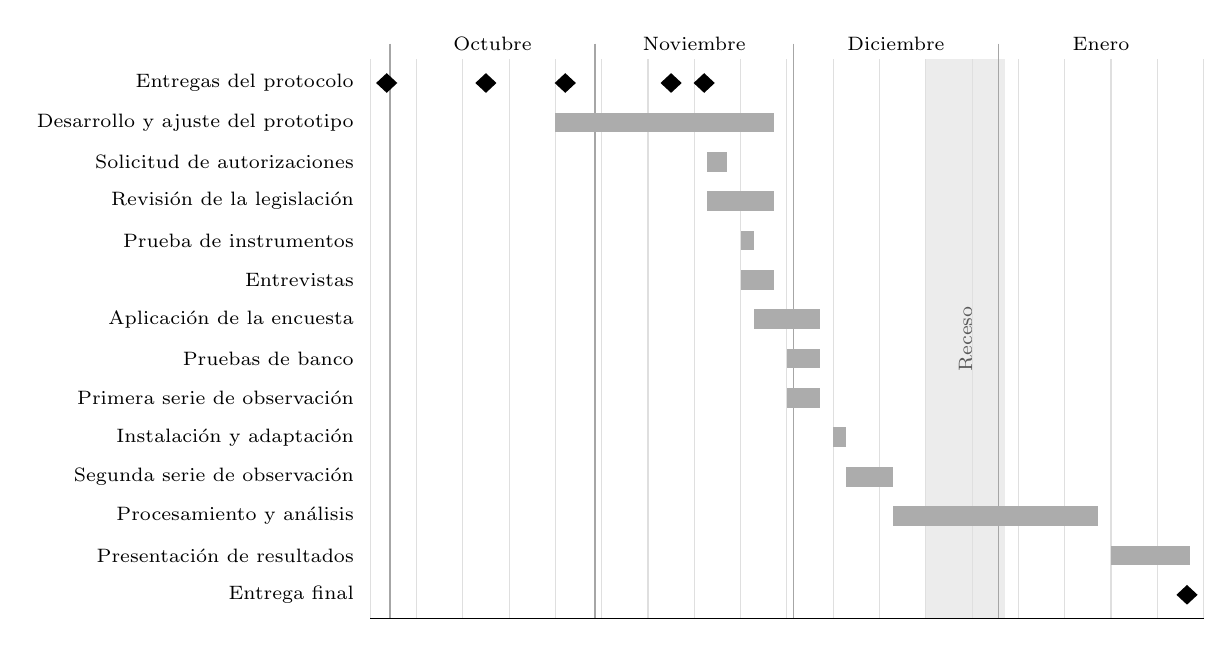
\begin{tikzpicture}[x=0.084cm,y=-0.5cm,font=\scriptsize]
		% Receso escolar (21 de diciembre al 1 de enero).
		\fill[gray!15] (84,0.4) rectangle (96,14.6);
		\node[gray!70!black,rotate=90] at (90,7.5) {Receso};
		% Cuadrícula semanal y meses.
		\foreach \d in {0,7,...,126} {\draw[gray!25] (\d,0.4) -- (\d,14.6);}
		\foreach \d in {3,34,64,95} {\draw[gray!70] (\d,0) -- (\d,14.6);}
		\node at (18.5,0) {Octubre};
		\node at (49,0) {Noviembre};
		\node at (79.5,0) {Diciembre};
		\node at (110.5,0) {Enero};
		\draw (0,14.6) -- (126,14.6);
		% Etiquetas de las actividades.
		\foreach \y/\t in {
				1/Entregas del protocolo,
				2/Desarrollo y ajuste del prototipo,
				3/Solicitud de autorizaciones,
				4/Revisión de la legislación,
				5/Prueba de instrumentos,
				6/Entrevistas,
				7/Aplicación de la encuesta,
				8/Pruebas de banco,
				9/Primera serie de observación,
				10/Instalación y adaptación,
				11/Segunda serie de observación,
				12/Procesamiento y análisis,
				13/Presentación de resultados,
				14/Entrega final} {
				\node[anchor=east,align=right] at (-1,\y) {\t};
			}
		% Hitos (rombos).
		\foreach \d in {2.5,17.5,29.5,45.5,50.5} {
				\fill (\d,0.75) -- (\d+1.6,1) -- (\d,1.25) -- (\d-1.6,1) -- cycle;
			}
		\fill (123.5,13.75) -- (125.1,14) -- (123.5,14.25) -- (121.9,14) -- cycle;
		% Barras: inicio y fin (día siguiente al último día de trabajo).
		\foreach \y/\a/\b in {
				2/28/61,
				3/51/54,
				4/51/61,
				5/56/58,
				6/56/61,
				7/58/68,
				8/63/68,
				9/63/68,
				10/70/72,
				11/72/79,
				12/79/110,
				13/112/124} {
				\fill[gray!65] (\a,\y-0.25) rectangle (\b,\y+0.25);
			}
	\end{tikzpicture}
	\figurenote{Elaboración propia con las fechas de la
		Tabla~\ref{tab:cronograma}. Las líneas verticales claras marcan el
		inicio de cada semana (lunes) y las oscuras el inicio de cada mes. Los
		rombos son entregas: planteamiento y objetivos, justificación, marco
		teórico, hipótesis, bosquejo del método y entrega final. La franja gris
		es el receso escolar.}
\end{figure}

Las actividades de la etapa 2 se encadenan de forma que ninguna dependa de
un resultado que todavía no existe. Las autorizaciones y la revisión de la
legislación van primero, porque sin ellas no se puede entrar al acceso ni
recabar datos personales. Las pruebas de banco coinciden con la primera serie
de observación: mientras se mide la línea base con la revisión visual de la
credencial, el prototipo se prueba fuera del acceso, y solo se instala si
cumple los criterios del Apéndice~E. El piloto termina el 15 de diciembre,
antes del receso, y la semana del 14 al 18 de diciembre queda como holgura
para repetir algún día de observación que se pierda. Si las autorizaciones
se retrasan, el trabajo de campo se recorre en bloque, pero la presentación
de resultados conserva su fecha y se reduce lo que se analiza antes que el
número de días observados.

\section{Presupuesto}
El presupuesto es una estimación preliminar hecha con precios de referencia
del mercado mexicano y se confirma al cotizar. No hay financiamiento externo:
lo cubren los seis integrantes del equipo, lo que equivale a unos 683 pesos
por persona. La Tabla~\ref{tab:presupuesto} desglosa cada partida, lo que
incluye y la etapa en que se ejerce.

\begin{table}[htbp]
	\caption{Presupuesto Estimado del Proyecto}
	\label{tab:presupuesto}
	\small\linespread{1}\selectfont\setlength{\tabcolsep}{3pt}
	\begin{tabular}{@{}P{3.6cm}P{6.6cm}P{3.6cm}r@{}}
		\toprule
		Partida & Incluye & Etapa en que se ejerce & Monto (MXN) \\
		\midrule
		Hardware del prototipo & Lector ESP32-CAM, placa ESP32, motor del torniquete, luces y zumbador, fuente de energía, base de MDF y cableado. & Desarrollo del prototipo & 1,750 \\[0.4em]
		Servidor, dominio y alojamiento & Servidor con la base de datos, dominio y alojamiento durante cuatro meses. & Desarrollo, piloto y análisis & 970 \\[0.4em]
		Impresiones y material de campo & Cuestionarios, hojas de observación, guías de entrevista, oficios, avisos de privacidad y formatos de consentimiento. & Trabajo de campo & 600 \\[0.4em]
		Traslados y compras & Traslados para comprar componentes y envíos. & Desarrollo del prototipo & 400 \\[0.4em]
		\midrule
		Subtotal & & & 3,720 \\
		Reserva de contingencia & Cerca del 10\,\% del subtotal, para reponer componentes dañados o precios mayores a los estimados. & Cualquier etapa & 380 \\
		\midrule
		Total estimado & & & 4,100 \\
		\bottomrule
	\end{tabular}
	\tablenote{Elaboración propia a partir del presupuesto del plan de gestión
		del proyecto. Las cerca de 800 horas de trabajo del equipo no se
		monetizan. Si el plantel presta el servidor, el total baja 970 pesos y
		queda en 3,130 pesos.}
\end{table}

Además del gasto en dinero, el proyecto usa recursos que no se compran. El
\tescha{} aporta el permiso para trabajar en el acceso, un espacio con
corriente eléctrica y red inalámbrica, el apoyo del personal de vigilancia y
el padrón de estudiantes de Control Escolar. Los integrantes aportan sus
computadoras, sus teléfonos y el entorno de programación, que se basa en
herramientas libres. Estos recursos no se suman al total porque no
representan una salida de dinero para el proyecto.

El gasto se controla con cuatro reglas: el presupuesto se aprueba antes de
la primera compra, cada compra se registra con su comprobante y su
responsable, una variación mayor de 10\,\% en una partida obliga a replantear
lo que se compra y el gasto acumulado se compara con lo planeado en la junta
semanal del equipo.
